\section{More Implementation Details}
The feature extractor for calculating $\mathcal{L}_\text{fidelity}$ is VGG16~\cite{Simonyan2014VeryDC} with IMAGENET1K-V1 checkpoint. We use the SDEdit with the forward step $t=500$ for our main study results as it balances faithfulness to the original image and flexibility for editing. Empirically, we choose to randomly sample the forward step $t \sim [0, 500]$ to enhance the optimization efficiency. The average time to optimize 300 steps for an image on a single Nvidia Tesla V100 is about 300 seconds. The estimated average memory usage is about 24GB. Table \ref{tab:step_size} provides the details of the step sizes that we use to attack different models. 

\begin{table}[h]
\footnotesize{
    \centering
    \begin{tabular}{lccc}
        \toprule
        \multirow{2}{*}{Models} & \multicolumn{2}{c}{Step Size} \\ 
         &  $\gamma_1$ ($\mathcal{L}_\text{attack}$)  & $\gamma_2$ ($\mathcal{L}_\text{fidelity}$)   \\
        \midrule
        google/ddpm-ema-church-256 & $100/255$ & $40/255$ \\
        google/ddpm-cat-256 & $100/255$ & $5/255$ \\
        google/ddpm-ema-celebahq-256 & $50/255$ & $35/255$ \\  
        
        \bottomrule
    \end{tabular}
    \caption{The step sizes used for different models during optimization.} 
\label{tab:step_size}
}
\end{table}


\section{More Experimental Results}

\subsection{Attack Effectiveness on Latent Diffusion Models}
We propose the feature representation attacking loss which can be adapted to target any UNet-based diffusion models. Hence, it is applicable to attack LDM using our proposed framework. We follow the evaluation settings of the previous works~\cite{xue2024effectiveprotectiondiffusionbased} for fair comparisons. Quantitative results are shown in Table~\ref{tab:attackLDM}. Compared to previous LDM-specified methods, our method could achieve comparable results. This finding reflects the general vulnerability in UNet-based diffusion models that can be exploited to craft adversarial images against either PDMs or LDMs. 

\begin{table*}[t]
    \centering
    \small{
    \begin{tabular}{ll|ccc|cccc}
        \toprule
        & \multirow{2}{*}{Methods} & \multicolumn{3}{c|}{Adversarial Image Quality} & \multicolumn{4}{c}{Attacking Effectiveness} \\ 
         & & SSIM $\uparrow$ & PSNR $\uparrow$ & LPIPS $\downarrow$ & SSIM $\downarrow$ & PSNR $\downarrow$ & LPIPS $\uparrow$ & IA-Score $\downarrow$ \\
        \midrule
        \multirow{6}{*}{\rotatebox{90}{Church}}
        & AdvDM ($+$) & \first{0.85} $\pm$ 0.03 & \first{30.42} $\pm$ 0.15 & \second{0.23} $\pm$ 0.06 & 0.19 $\pm$ 0.05 & 28.00 $\pm$ 0.16 & 0.71 $\pm$ 0.04 & 0.49 $\pm$ 0.06 \\
        & Mist ($+$) & 0.81 $\pm$  0.03 & 29.45 $\pm$ 0.13 & 0.25 $\pm$ 0.05 & \first{0.14} $\pm$ 0.03 & \first{27.95} $\pm$ 0.13 & \first{0.76} $\pm$ 0.04 & \second{0.48} $\pm$ 0.05 \\
        & Diff-Protect ($-$) & 0.79 $\pm$ 0.03 & 29.92 $\pm$ 0.15 & 0.24 $\pm$ 0.06 & \second{0.15} $\pm$ 0.03 & 28.00 $\pm$ 0.14 & 0.71 $\pm$ 0.04 & \second{0.48} $\pm$ 0.05 \\
        & Diff-Protect ($+$) & 0.79 $\pm$ 0.04 & 29.47 $\pm$ 0.11 & 0.26 $\pm$ 0.06 & 0.17 $\pm$ 0.04 & 28.00 $\pm$ 0.15 & 0.69 $\pm$ 0.04 & 0.49 $\pm$ 0.06 \\
        & AtkPDM (Ours) & \second{0.82} $\pm$ 0.02 & \second{30.40} $\pm$ 0.27 & 0.24 $\pm$ 0.05 & \first{0.14} $\pm$ 0.03 & \second{27.96} $\pm$ 0.17 & \second{0.74} $\pm$ 0.02 & \first{0.47} $\pm$ 0.04  \\
        & AtkPDM$^+$ (Ours) & 0.61 $\pm$ 0.07 & 29.17 $\pm$ 0.32 & \first{0.20} $\pm$ 0.02 & 0.27 $\pm$ 0.06 & 28.07 $\pm$ 0.18 & 0.66 $\pm$ 0.05 & 0.51 $\pm$ 0.06 \\
        \midrule
        \multirow{6}{*}{\rotatebox{90}{Cat}}
        & AdvDM ($+$) & \first{0.86} $\pm$ 0.04 & \second{30.68} $\pm$ 0.24 & \second{0.25} $\pm$ 0.09 & 0.21 $\pm$ 0.05 & 28.03 $\pm$ 0.21 & 0.70 $\pm$ 0.07 & \second{0.53} $\pm$ 0.04 \\
        & Mist ($+$) & 0.81 $\pm$ 0.04 & 29.63 $\pm$ 0.22 & 0.27 $\pm$ 0.08 & \first{0.14} $\pm$ 0.04 & \first{27.96} $\pm$ 0.17 & \first{0.77} $\pm$ 0.06 & \first{0.52} $\pm$ 0.04 \\
        & Diff-Protect ($-$) & 0.78 $\pm$ 0.05 & 30.12 $\pm$ 0.24 & 0.27 $\pm$ 0.08 & \second{0.16} $\pm$ 0.05 & \first{27.96} $\pm$ 0.15 & \second{0.72} $\pm$ 0.06 & \first{0.52} $\pm$ 0.03 \\
        & Diff-Protect ($+$) & 0.77 $\pm$ 0.06 & 29.56 $\pm$ 0.16 & 0.28 $\pm$ 0.09 & 0.17 $\pm$ 0.05 & \second{27.98} $\pm$ 0.16 & 0.71 $\pm$ 0.06 & \second{0.53} $\pm$ 0.04 \\
        & AtkPDM (Ours) & \second{0.84} $\pm$ 0.02 & \first{30.79} $\pm$ 0.49 & \second{0.25} $\pm$ 0.07 & 0.18 $\pm$ 0.04 & 28.00 $\pm$ 0.19 & \second{0.72} $\pm$ 0.05 & \first{0.52} $\pm$ 0.03  \\
        & AtkPDM$^+$ (Ours) & 0.68 $\pm$ 0.13 & 29.68 $\pm$ 0.74 & \first{0.16} $\pm$ 0.03 & 0.31 $\pm$ 0.10 & 28.13 $\pm$ 0.27 & 0.64 $\pm$ 0.06 & 0.54 $\pm$ 0.04 \\
        \midrule
        \multirow{6}{*}{\rotatebox{90}{Face}}
        & AdvDM ($+$) & \first{0.83} $\pm$ 0.02 & \second{30.81} $\pm$ 0.22 & 0.32 $\pm$ 0.06 & 0.26 $\pm$ 0.05 & 28.07 $\pm$ 0.28 & 0.74 $\pm$ 0.05 & 0.47 $\pm$ 0.07 \\
        & Mist ($+$) & 0.79 $\pm$ 0.03 & 29.75 $\pm$ 0.22 & 0.34 $\pm$ 0.06 & \first{0.19} $\pm$ 0.05 & \first{27.99} $\pm$ 0.21 & \first{0.81} $\pm$ 0.05 & 0.46 $\pm$ 0.08 \\
        & Diff-Protect ($-$) & 0.74 $\pm$ 0.04 & 30.34 $\pm$ 0.13 & 0.33 $\pm$ 0.06 & \second{0.21} $\pm$ 0.05 & \second{28.03} $\pm$ 0.21 & 0.76 $\pm$ 0.06 & \second{0.45} $\pm$ 0.07 \\
        & Diff-Protect ($+$) & 0.72 $\pm$ 0.05 & 29.68 $\pm$ 0.09 & 0.36 $\pm$ 0.06 & \second{0.21} $\pm$ 0.04 & 28.05 $\pm$ 0.22 & 0.74 $\pm$ 0.06 & 0.47 $\pm$ 0.07 \\
        & AtkPDM (Ours) & \first{0.83} $\pm$ 0.02 & \first{31.21} $\pm$ 0.44 & \second{0.31} $\pm$ 0.05 & \second{0.21} $\pm$ 0.04 & \second{28.03} $\pm$ 0.26 & \second{0.78} $\pm$ 0.04 & \first{0.44} $\pm$ 0.06  \\
        & AtkPDM$^+$ (Ours) & \second{0.82} $\pm$ 0.05 & 30.05 $\pm$ 0.51 & \first{0.14} $\pm$ 0.03 & 0.41 $\pm$ 0.08 & 28.24 $\pm$ 0.39 & 0.63 $\pm$ 0.07 & 0.52 $\pm$ 0.07 \\
        \bottomrule
    \end{tabular}
    }
    \caption{Quantitative results in attacking LDM.}
    \label{tab:attackLDM}
\end{table*}


\subsection{Qualitative Demonstration of Corrupting UNet Feature during Sampling}
We qualitatively show an example of our attack effectiveness regarding UNet representation discrepancies in Figure~\ref{fig:feature_visulization}. We compare a clean and an adversarial image using the same denoising process. Then, we take the feature maps of the second-last decoder block layer, close to the final predicted noise, to demonstrate their recognition of input image semantics.
The results in Figure~\ref{fig:feature_visulization} show that from $t$ = 500, the feature maps of each pair start with a similar structure, then as the $t$ decreases, the feature maps gradually have higher discrepancies, suggesting our method, by attacking the middle representation of UNet, can effectively disrupt the reverse denoising process and mislead to corrupted samples.

\begin{figure*}[h]
\centering
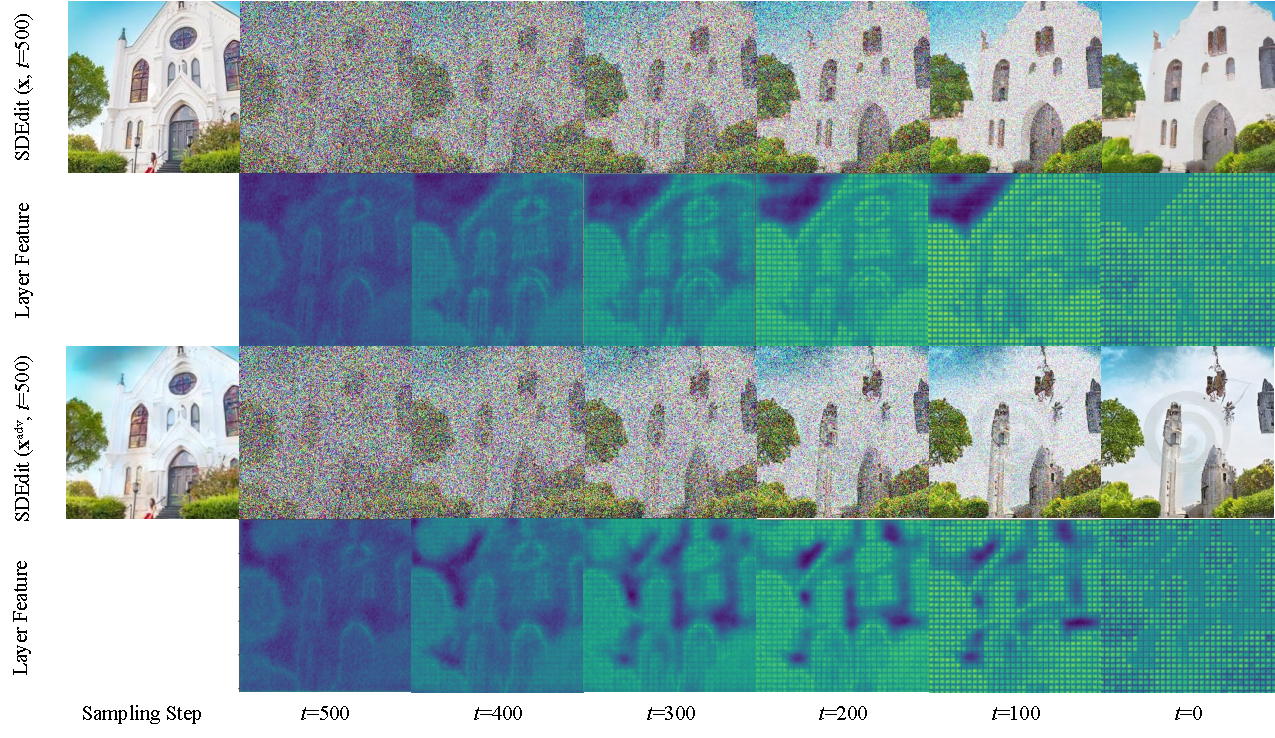
\includegraphics[width=0.9\linewidth]{figures/feature_visulization.pdf}
\caption{Qualitative example of corrupting feature representations in UNet: as the denoising process proceeds, the similarity of the feature map decreases, suggesting the representation is corrupted.}
\label{fig:feature_visulization}
\end{figure*}

\subsection{Qualitative Results of Loss Ablation}
Figure~\ref{fig:loss_ablation} presents qualitative results of loss ablation where i., ii., and iii. indicate performing PGAscent with different configurations. i. utilizes only semantic loss; ii. utilizes semantic loss with our latent optimization strategy; iii. utilizes both semantic loss, our proposed $\mathcal{L}_\text{fidelity}$ and latent optimization. The results show that our $\mathcal{L}_\text{fidelity}$ and latent optimization can enhance the adversarial image quality of PGAscent. Moreover, comparing our proposed two methods, AtkPDM$^+$ generates a more natural adversarial image than AtkPDM while maintaining attack effectiveness.

\begin{figure*}[h]
\centering
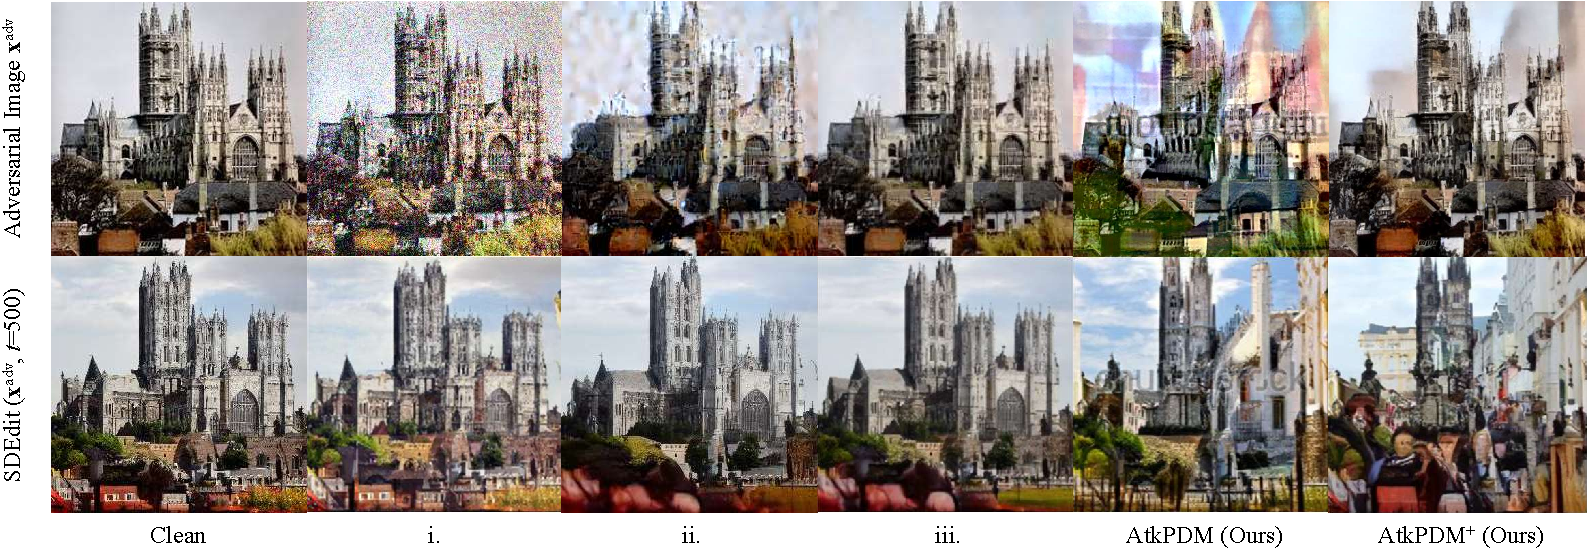
\includegraphics[width=1\linewidth]{figures/loss_ablation.pdf}
\caption{Qualitative example of different loss configurations. i. only semantic loss; ii. semantic loss and latent optimization; iii. semantic loss, $\mathcal{L}_\text{fidelity}$ and latent optimization.}
\label{fig:loss_ablation}
\end{figure*}

\subsection{Different Forward Time-step Sampling}

When using Monte Carlo sampling for optimization, the forward time step $t^*$ is sampled uniformly. We study the scenario that when $t^*$ is fixed for optimization. As shown in Figure~\ref{fig:different_timestep}, a primary result shows that when attacking $t^*=400$ to $t^*=500$, the attacking effectiveness is better than other time steps. In practice, we can not know user-specified $t^*$ for editing in advance; however, this suggests that diffusion models have a potential temporal vulnerability that can be further exploited to increase efficiency.

\begin{figure*}[h]
\centering
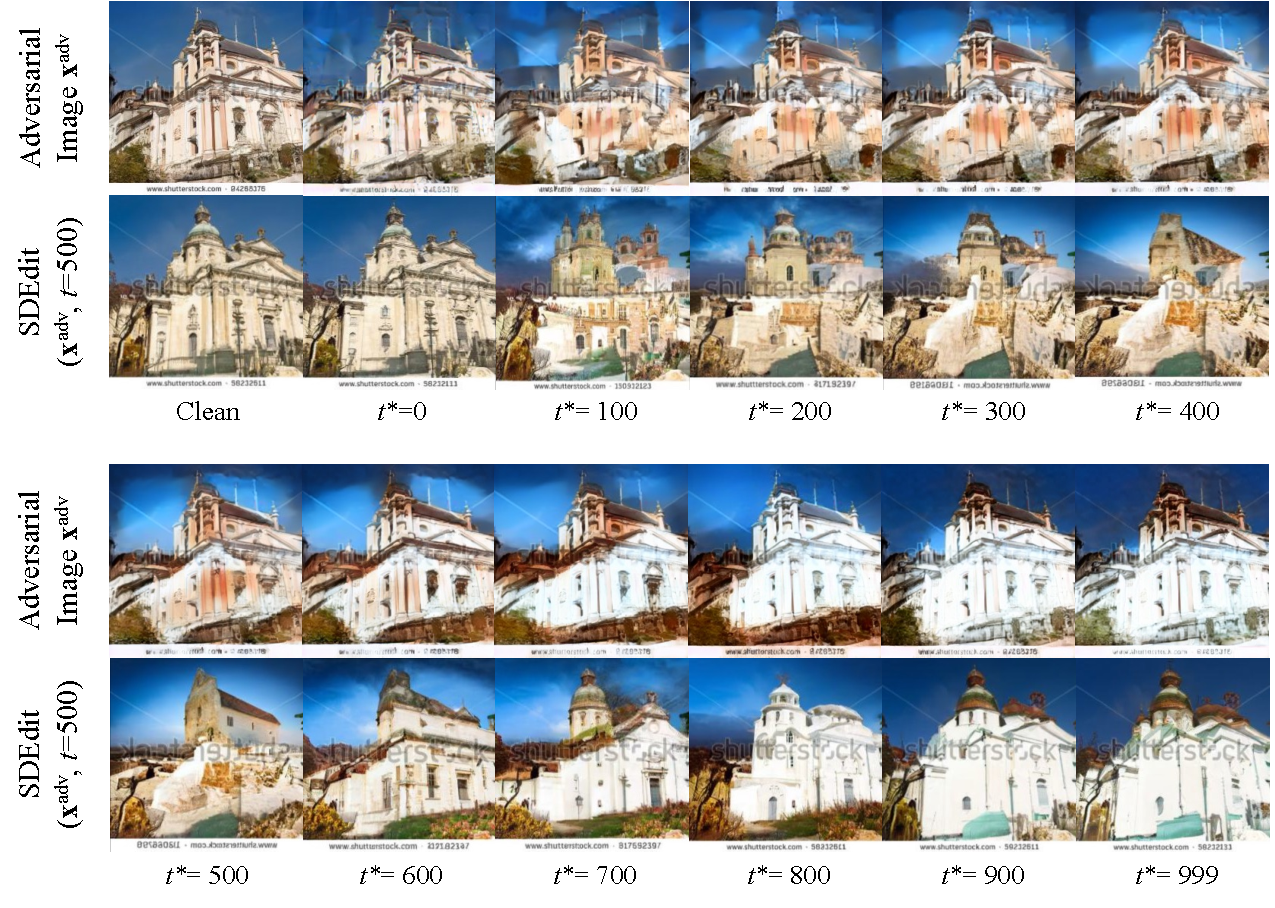
\includegraphics[width=0.9\linewidth]{figures/different_timestep.pdf}
\caption{Qualitative results of optimizing different fixed diffusion forward steps.}
\label{fig:different_timestep}
\end{figure*}

\subsection{More Qualitative Results}
We provide more qualitative results in Figure~\ref{supp:qualitative} to showcase that our method can significantly change or corrupt the generated results with little modification on adversarial images. In contrast, previous methods add obvious perturbation to adversarial images but still fail to change the edited results to achieve the safeguarding goal.

\begin{figure*}
\centering
\begin{subfigure}{1\linewidth}
    \centering
    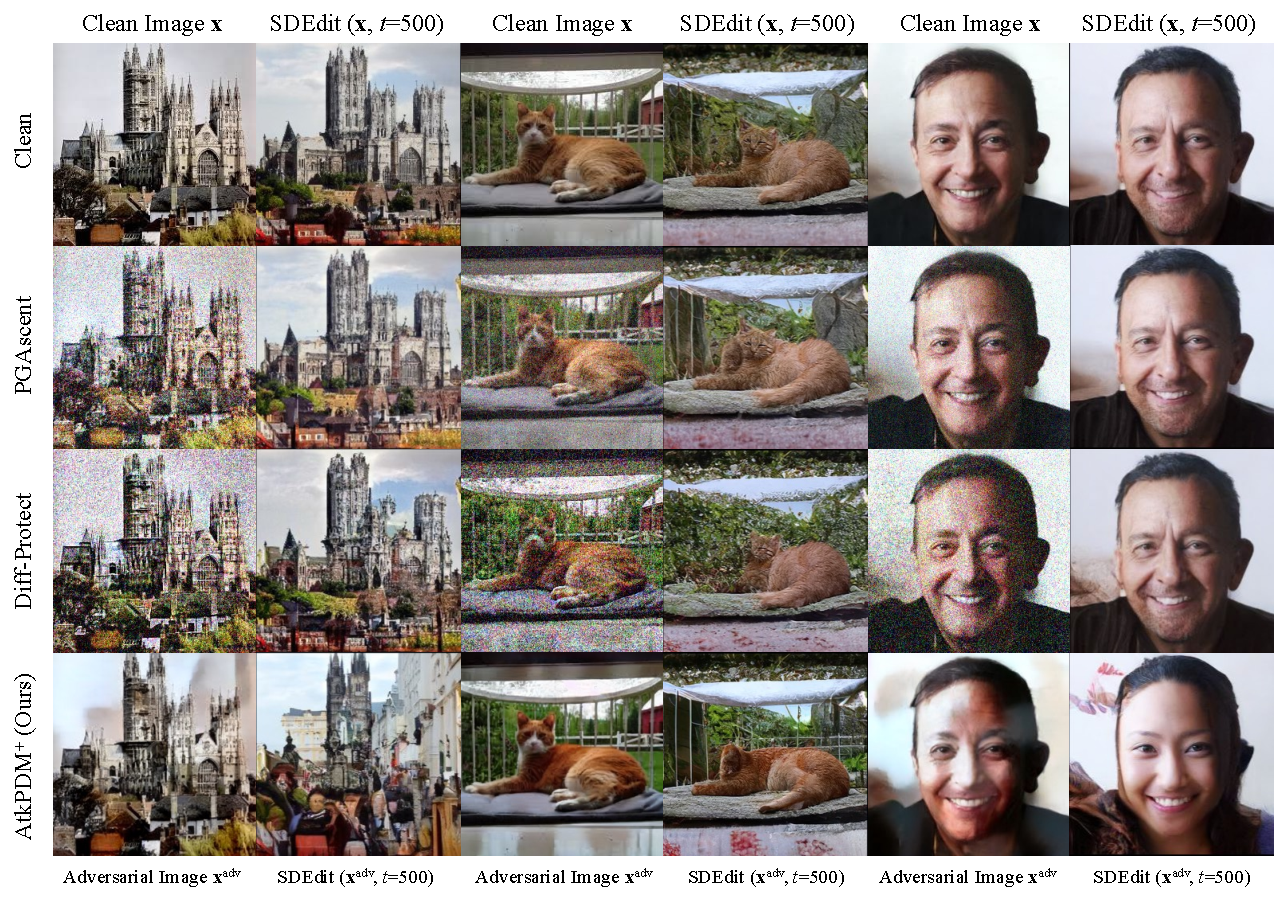
\includegraphics[width=0.9\linewidth]{figures/qualitative_results_1.pdf}
    \label{fig:qualitative_results_1}
\end{subfigure}

\begin{subfigure}{0.9\linewidth}
    \centering
    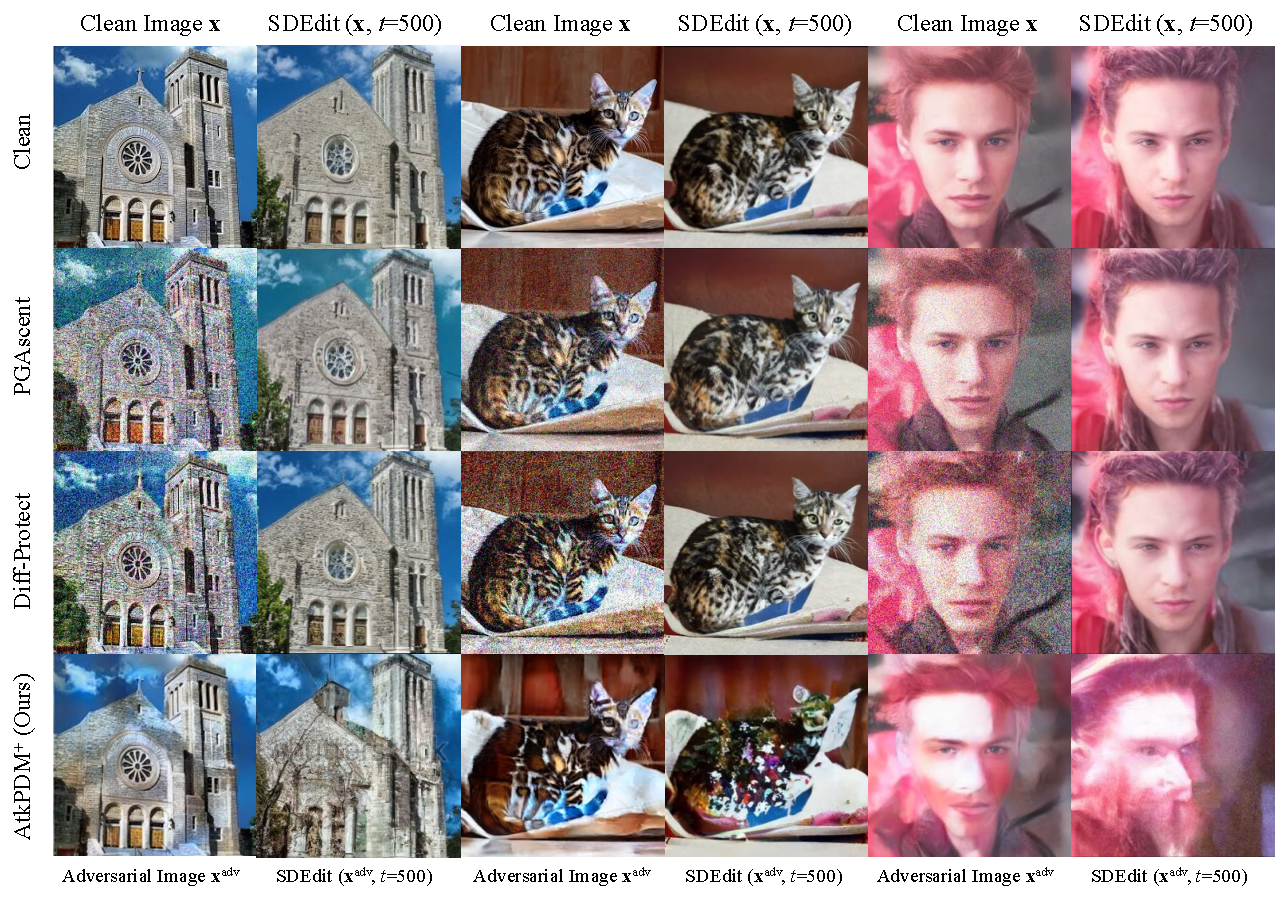
\includegraphics[width=1\linewidth]{figures/qualitative_results_2.pdf}
    \label{fig:qualitative_results_2}
\end{subfigure}
\caption{Qualitative results compared to previous methods: our adversarial images can effectively corrupt the edited results without significant fidelity decrease. The same column shares the same random seed for fair comparison.}
\label{supp:qualitative}
\end{figure*}

\subsection{Example of Loss Curves}

Figure \ref{supp:loss_curve} shows an example of our loss trends among optimization steps. $\mathcal{L}_\text{attack}$ has decreasing trend as the optimization step increases. $\mathcal{L}_\text{fidelity}$ has an increasing trend and converges to satisfy the constraint of the attack budget $\delta$.

\section{Limitations}
While our method can deliver acceptable attacks on PDMs, its visual quality is still not directly comparable to the results achieved on LDMs, indicating room for further improvement. More generalized PDM attacks should be further explored. 

\section{Societal Impacts}
Our work will not raise potential concerns about diffusion model abuses. Our work is dedicated to addressing these issues by safeguarding images from being infringed.

\begin{figure*}
\centering
\begin{subfigure}{1\linewidth}
    \centering
    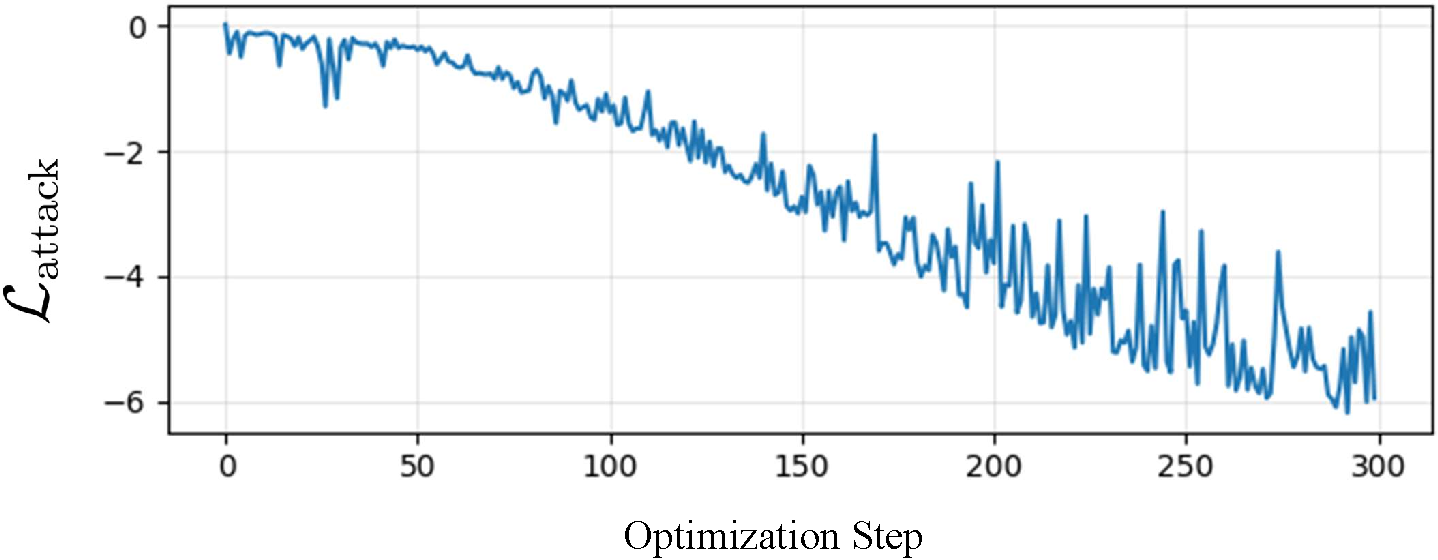
\includegraphics[width=0.7\linewidth]{figures/attack_loss_curve.pdf}
    \label{fig:attack_loss_curve}
\end{subfigure}

\begin{subfigure}{1\linewidth}
    \centering
    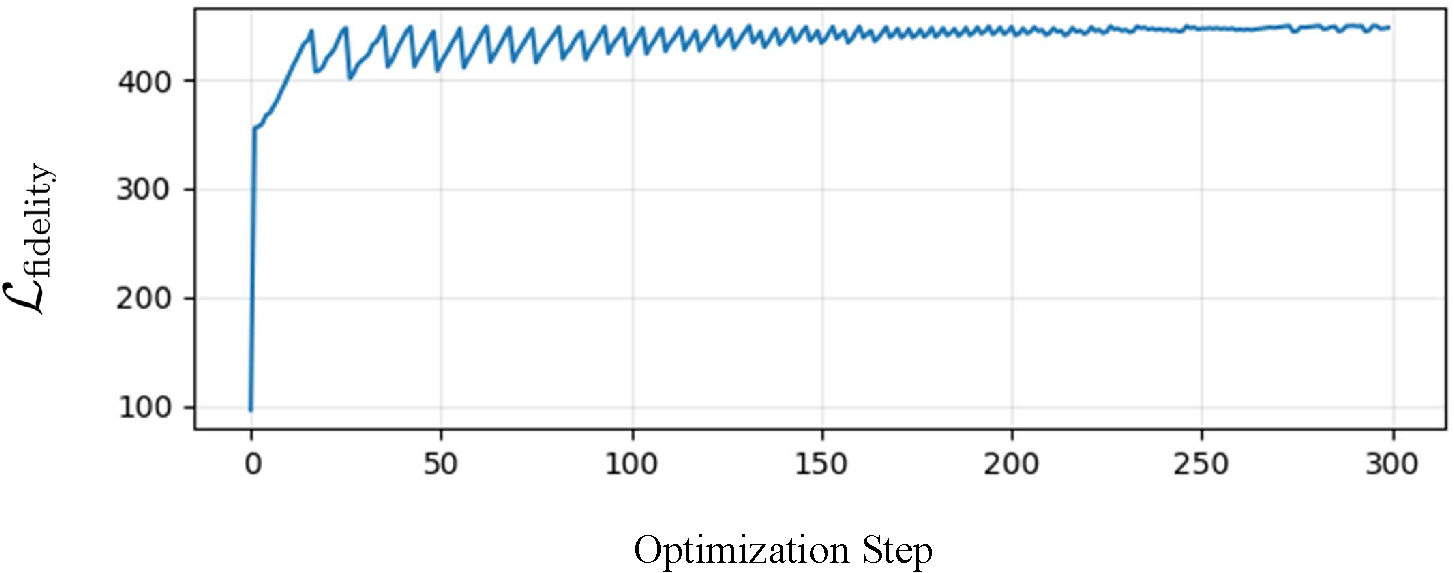
\includegraphics[width=0.7\linewidth]{figures/fidelity_loss_curve.pdf}
    \label{fig:fidelity_loss_curve}
\end{subfigure}
\caption{Loss curves of our $\mathcal{L}_\text{attack}$ and $\mathcal{L}_\text{fidelity}$ against optimization step.}
\label{supp:loss_curve}
\end{figure*}

\section{Details of Our Proposed Algorithm}

\subsection{AtkPDM Algorithm without Latent Optimization}

\begin{algorithm}[H]
    \caption{AtkPDM}
    \label{alg:attdpm}
    \small{
    \begin{algorithmic}[1] 
        \STATE{\textbf{Input:}
        Image to be protected $\mathbf{x}$, attack budget $\delta > 0$, and step size $\gamma_1, \gamma_2>0$}
        \STATE{\textbf{Initialization:} $\mathbf{x}^{\adv} \leftarrow \mathbf{x}$, $L_\text{attack} \leftarrow \infty$}
        \WHILE{$L_\text{attack}$ not convergent}
            \STATE{Sample timestep: $t \sim [0, T]$}
            \STATE{Sample noise: $\epsilon_1, \epsilon_2 \sim \normaldist$}
            \STATE{Compute original noisy sample: $\mathbf{x}_t \leftarrow \mathcal{F}(\mathbf{x}, t, \epsilon_1)$}
            \STATE{Compute adversarial noisy sample: $\mathbf{x}^{\adv}_t \leftarrow \mathcal{F}(\mathbf{x}^{\adv}, t, \epsilon_2)$}
            \STATE{Update $\mathbf{x}^{\adv}$ by Gradient Descent: \\
            $\mathbf{x}^{\adv} \leftarrow \mathbf{x}^{\adv} -
            \gamma_1 \sign(\nabla_{\mathbf{x}^{\adv}} \mathcal{L}_\text{attack}(\mathbf{x}^{\adv}_t, {\mathbf{x}_t}))$}            \WHILE{$\mathcal{L}_\text{fidelity}(\mathbf{x}^{\adv}, \mathbf{x}) > \delta$}
            \STATE{$\mathbf{x}^{\adv} \leftarrow \mathbf{x}^{\adv} -
            \gamma_2 \nabla_{\mathbf{x}^{\adv}} \mathcal{L}_\text{fidelity}(\mathbf{x}^{\adv}, \mathbf{x})$}
            \ENDWHILE
        \ENDWHILE
        \RETURN {$\mathbf{x}^{\adv}$}
    \end{algorithmic}
    }
\end{algorithm}


\subsection{2-Wasserstein Distance Between Two Normal Distribution}
Consider the normal distributions $\mathcal{N}_t:=\mathcal{N}(\mu_t, \Sigma_t)$ and $\mathcal{N}_t^{\adv}:=\mathcal{N}(\mu_t^{\adv}, \Sigma_t^{\adv})$. Let $\Pi(\mathcal{N}_t, \mathcal{N}_t^{\adv})$ denote a joint distribution over the product space $\mathbb{R}^n \times \mathbb{R}^n$. The 2-Wasserstein distance between $\mathcal{N}_t$ and $\mathcal{N}_t^{\adv}$ is defined as:
\begin{align*}
    \mathcal{W}_2^2(\mathcal{N}_t, \mathcal{N}_t^{\adv})
    =\min_{\pi \in \Pi(\mathcal{N}_t, \mathcal{N}_t^{\adv})} \int \|\mathbf{x}_t-\mathbf{x}_t^{\adv}\|_2^2 \text{d}\pi(\mathbf{x}_t, \mathbf{x}_t^{\adv}).
\end{align*}

Using properties of the mean and covariance, we have the following identities:
\begin{align*}
    &\int \|\mu_t-\mu_t^{\adv}\|_2^2 \text{d}\pi(\mathbf{x}_t, \mathbf{x}_t^{\adv}) = \|\mu_t-\mu_t^{\adv}\|_2^2, \\
    &\int \|\mathbf{x}_t-\mu_t\|_2^2 \text{d}\pi(\mathbf{x}_t, \mathbf{x}_t^{\adv}) = \trac(\Sigma_t), \\
    &\int \|\mathbf{x}_t^{\adv}-\mu_t^{\adv}\|_2^2 \text{d}\pi(\mathbf{x}_t, \mathbf{x}_t^{\adv}) = \trac(\Sigma_t^{\adv}), \\
    &\int (\mathbf{x}_t-\mu_t)^\top(\mathbf{x}_t^{\adv}-\mu_t^{\adv}) \text{d}\pi(\mathbf{x}_t, \mathbf{x}_t^{\adv}) \\
    &=\trac\left(\mathbb{E}[(\mathbf{x}_t-\mu_t)(\mathbf{x}_t^{\adv}-\mu_t^{\adv})^\top\right).
\end{align*}
Thus, the 2-Wasserstein distance can be expressed as:
\begin{equation}
\begin{aligned}
    \mathcal{W}_2^2(\mathcal{N}_t, \mathcal{N}_t^{\adv})
    &=\|\mu_t-\mu_t^{\adv}\|_2^2 \\
    + \trac{(\Sigma_t)} &+ \trac{(\Sigma_t^{\adv})}
    -2\max_{J \succeq 0} \trac(C),
\end{aligned}
\end{equation}
where $J$ is the joint covariance matrix of $\mathcal{N}_t$ and $\mathcal{N}_t^{\adv}$, defined as:
\begin{align*}
J = \left[
\begin{array}{cc}
    \Sigma_t & C \\
    C^\top   & \Sigma_t^{\adv}
\end{array}
\right],
\end{align*}
and $C$ is the covariance matrix between $\mathcal{N}_t$ and $\mathcal{N}_t^{\adv}$:
\begin{align*}
C = \mathbb{E}
\left[
(\mathbf{x}_t-\mu_t)(\mathbf{x}_t^{\adv}-\mu_t^{\adv})^{\top}
\right].
\end{align*}

By the Schur complement, the problem can be formulated as a semi-definite programming (SDP) problem:
\begin{equation}
\begin{aligned}
&\text{maximum} \quad \trac(C), \\
&\text{subject to } \quad
\Sigma_t - C^\top (\Sigma_t^{\adv})^{-1} C \succeq 0.
\end{aligned}
\end{equation}
The closed-form solution for $C$ derived from the SDP is:
\begin{equation*}
    C=
    \Sigma_t^{\frac{1}{2}}
    (\Sigma_t^{\frac{1}{2}}\Sigma_t^{\adv}\Sigma_t^{\frac{1}{2}})^\frac{1}{2}
    \Sigma_t^{-\frac{1}{2}}.
\end{equation*}

Finally, the closed-form solution for the 2-Wasserstein distance between the two normal distributions is given by:
\begin{equation}
\begin{aligned}
    \mathcal{W}_2^2(\mathcal{N}_t, \mathcal{N}_t^{\adv})
    &=\|\mu_t-\mu_t^{\adv}\|_2^2 \\
    + \trac{(\Sigma_t)} &+ \trac{(\Sigma_t^{\adv})}
    -2(\Sigma_t^{\frac{1}{2}}\Sigma_t^{\adv}\Sigma_t^{\frac{1}{2}})^\frac{1}{2}.
\end{aligned}
\end{equation}


\subsection{Alternating Optimization}
Let $\mathbf{y} = \mathbf{x}^{\adv}$, by Lagrange relaxation \cite{liu2023instruct2attack}, the objective function can be expressed as:    
\begin{equation}
F(\mathbf{x}, \mathbf{y}) = F_1(\mathbf{x}, \mathbf{y}) + \lambda F_2(\mathbf{x}, \mathbf{y}),
\end{equation}
where $\lambda > 0$ is the Lagrange multiplier and $F_1$, $F_2$ are defined as
\begin{align}
    F_1(\mathbf{x}, \mathbf{y})
    &=\mathcal{L}_\text{attack}(
    \mathcal{F}(\mathbf{x}, t, \epsilon_1), \mathcal{F}(\mathbf{y}, t, \epsilon_2)), \\
    F_2(\mathbf{x}, \mathbf{y})
    &=\max (\epsilon-\mathcal{L}_\text{fidelity}(\mathbf{x}, \mathbf{y}), \mathbf{0}).
\end{align}

The optimization is carried out in an alternating manner as follows:
\begin{align}
    & \mathbf{y}^{i+\frac{1}{2}} = \argmin_{\mathbf{y}} \left(F_1(\mathbf{x}, \mathbf{y}) + \lambda F_2(\mathbf{x}, \mathbf{y}^{i})\right), \label{eq:F1} \\
    & \mathbf{y}^{i+1} = \argmin_{\mathbf{y}} \left(F_1(\mathbf{x}, \mathbf{y}^{i+\frac{1}{2}}) + \lambda F_2(\mathbf{x}, \mathbf{y})\right). \label{eq:F2}
\end{align}

To solve Equation \ref{eq:F1}, we employ the Fast Gradient Sign Method (FGSM) \cite{ian2015fgsm}. The update is given by:
\begin{equation}
\mathbf{y}^{i+1/2} = \mathbf{y}^{i} - \gamma_1 \sign\left(\nabla_{\mathbf{y}^i} F_1(\mathbf{x}, \mathbf{y}^i)\right),
\end{equation}

For Equation \ref{eq:F2}, we utilize Gradient Descent, resulting in the following update:
\begin{align}
\mathbf{y}^{i+1} = \mathbf{y}^{i+\frac{1}{2}} - \Tilde{\gamma}_2 \nabla_{\mathbf{y}^{i+\frac{1}{2}}} \lambda F_2(\mathbf{x}, \mathbf{y}^{i+\frac{1}{2}}) \\
= \mathbf{y}^{i+\frac{1}{2}} - \gamma_2 \nabla_{\mathbf{y}^{i+\frac{1}{2}}} F_2(\mathbf{x}, \mathbf{y}^{i+\frac{1}{2}}).
\end{align}
Note that the gradient of $F_2$ can be derived as follows:
\begin{align*}
    \nabla_{\mathbf{y}} F_2(\mathbf{x}, \mathbf{y})
    = \mathbb{I}_\mathcal{C'} \odot
    \nabla_{\mathbf{x}^{\adv}_t} \mathcal{L}_\text{fidelity}(\mathbf{x}, \mathbf{y}),
\end{align*}
where $\mathbb{I}_\mathcal{C'}$ is indicator function with constraint $\mathcal{C} = {\{\mathbf{y} \in \mathcal{M} \mid \mathcal{L}_\text{fidelity}(\mathbf{x}, \mathbf{y}) \leq \epsilon\}}$.\\

Please note that after references, we also provide more results presented in Figures~\ref{fig:loss_ablation}, ~\ref{fig:different_timestep}, ~\ref{supp:qualitative}, and~\ref{supp:loss_curve}, please refer to subsequent pages.

